\documentclass[12pt, aspectratio=169]{beamer}

\usetheme{moloch}
\molochset{block=fill}

\usepackage{fontspec}
\setsansfont[
    UprightFont = Inter-Light,          % Use light as the normal font weight
    BoldFont = Inter-SemiBold,           % Use semibold for \textbf
    ItalicFont = Inter-LightItalic,      % Light italic for \textit
    BoldItalicFont = Inter-SemiBoldItalic % Semibold italic for \textbf with \textit
]{Inter}[RawFeature={+ss04, +ss03, +dlig, +tnum}]
% Inter font stylistic sets:
% ss01: alternate digits for 3, 4, 6, 8
% ss02: for disambiguation (with zero) in places like "Ill" or "O0" etc
% ss04: for disambiguation (without zero) in places like "Ill" etc
% ss03: round comma, quation marks

\usepackage{upquote}
\usepackage{microtype}
\UseMicrotypeSet[protrusion]{basicmath}    % disable protrusion for tt fonts

\usepackage{amsmath}
\usepackage{amssymb}
\usepackage{unicode-math}
\setmathfont{Erewhon Math}[Scale=1.14]

\usepackage{hyperref}
\pdfstringdefDisableCommands{\def\translate#1{#1}}
\usepackage{bookmark}
\usepackage{url}

\usepackage{natbib}
\usepackage{appendixnumberbeamer}
\usepackage{enumerate}
% \usepackage{enumitem}    % it is giving the error: TeX capacity exceeded
% \usepackage{footnotehyper}
\usepackage{graphicx}
\usepackage{caption}
% \usepackage{subcaption}
\usepackage{booktabs}
\usepackage{makecell}
\usepackage{array}
\newcolumntype{H}{>{\setbox0=\hbox\bgroup\let\pm\relax}c<{\egroup}@{}}
% \newcolumntype{H}{>{\setbox0=\hbox\bgroup}c<{\egroup}}% <--- removed @{}
% https://tex.stackexchange.com/questions/567724/can-i-hide-a-table-column-with-the-s-type-from-siunitx
% https://tex.stackexchange.com/questions/414143/hide-column-without-adding-whitespace-to-table


\definecolor{airforceblue}{rgb}{0.36, 0.54, 0.66}
\hypersetup{
    colorlinks=true,
    linkcolor={mDarkTeal},    % this colour is defined by the moloch theme
    filecolor={Maroon},
    citecolor={airforceblue!120},
    urlcolor={airforceblue!140},
    pdfcreator={xelatex},
    bookmarksopen=true,    % Expand bookmarks in the PDF
    bookmarksnumbered=true % Include numbering in bookmarks
}

\bibliographystyle{apalike}

\let\oldcite=\cite
\renewcommand{\cite}[1]{\textcolor{airforceblue!120}{\oldcite{#1}}}
\let\oldcitet=\citet
\renewcommand{\citet}[1]{\textcolor{airforceblue!120}{\oldcitet{#1}}}
\let\oldcitep=\citep
\renewcommand{\citep}[1]{\textcolor{airforceblue!120}{\oldcitep{#1}}}


% \setlength{\leftmargini}{0em}
\setbeamercolor{page number in head/foot}{fg=gray}
\setbeamertemplate{footline}[frame number]
\setbeamertemplate{itemize items}[circle]
\setbeamertemplate{enumerate items}[circle]
\setbeamertemplate{sections/subsections in toc}[circle]
\setbeamertemplate{frametitle continuation}[from second][(cont.)]
\setbeamercovered{transparent}
\beamertemplatenavigationsymbolsempty


\AtBeginSubsection[]{
    {
        \begin{frame}[noframenumbering, plain]
            \subsectionpage
        \end{frame}
    }
}


\newcommand\Wider[2][4em]{%
    \makebox[\linewidth][c]{%
        \begin{minipage}{\dimexpr\textwidth+#1\relax}
            % \raggedright#2
            \centering#2
        \end{minipage}%
    }%
}

% \newenvironment{myitemize}{
%     \begin{itemize}
%         \vspace{1em}
%         \setlength{\itemsep}{0.7\baselineskip}
% }{
%         \vspace{1em}
%     \end{itemize}
% }

% \newenvironment{myenumerate}{
%     \begin{enumerate}
%         \vspace{1em}
%         \setlength{\itemsep}{0.7\baselineskip}
% }{
%         \vspace{1em}
%     \end{enumerate}
% }
\usepackage{tikz}
\usetikzlibrary{shapes.geometric, arrows}

% Define flowchart block styles (formal colors)
\tikzstyle{startstop} = [ellipse, minimum width=1cm, minimum height=1cm,
    text centered, draw=black, fill=red!20]
\tikzstyle{process} = [rectangle, minimum width=2cm, minimum height=1cm,
    text centered, draw=black, fill=blue!20]
\tikzstyle{decision} = [diamond, aspect=2,
    text centered, draw=black, fill=green!20]
\tikzstyle{io} = [trapezium, trapezium left angle=70, trapezium right angle=110,
    minimum width=2cm, minimum height=0.75cm, text centered, draw=black, fill=orange!20]
\tikzstyle{arrow} = [thick,->,>=stealth]

\title{Conditional Execution and Loops in C}
\author{}
\date{}

\begin{document}

    {
		\setbeamertemplate{footline}{}    % NO FOOTLINE FOR THESE TWO FRAMES
		\addtocounter{framenumber}{-2}    % not counting the title page and the outline in frame numbers

		\begin{frame}
			\titlepage
		\end{frame}

		\begin{frame}{Outline}
            % \vfill
            \small
			\tableofcontents[subsectionstyle=hide]
            % \vfill
		\end{frame}
	}

    \section{Conditional Execution}

    \begin{frame}{Conditional Execution in C}
        \begin{itemize}
            \item \textbf{Conditional execution} allows a program to take different actions based on certain conditions
            \item Conditions are expressed using \texttt{if}, \texttt{else}, and \texttt{else if} statements
            \item Condition expressions must evaluate to \texttt{true (non-zero)} or \texttt{false (zero)}
        \end{itemize}
    \end{frame}


    \begin{frame}[fragile]{\texttt{if} Statement}
        \textbf{Syntax:}
        \begin{verbatim}
if(condition){
    // statements
}
        \end{verbatim}

        \textbf{Example:}
        \inputminted[
            frame=none,
            bgcolor=gray!20,
            linenos, 
            breaklines=true,
            fontsize=\fontsize{12pt}{13pt}\selectfont,
            % firstline=1,
            % lastline=7,
            % firstnumber=1
        ]{c}{../code-examples/06_01_check-positive.c}
    \end{frame}


    \begin{frame}[fragile]{\texttt{if-else} Statement}
        \begin{verbatim}
if(condition){
    // commands to execute if true
} else{
    // commands to execute if false
}
        \end{verbatim}

    \end{frame}


    \begin{frame}[fragile]{\texttt{if-else} Example}
        \inputminted[
            frame=none,
            bgcolor=gray!20,
            linenos, 
            breaklines=true,
            fontsize=\fontsize{12pt}{13pt}\selectfont
        ]{c}{../code-examples/06_02_check-voter.c}
    \end{frame}


    \begin{frame}[fragile]{\texttt{else if} Ladder}
        \begin{verbatim}
if(condition1){
    ...
} else if(condition2) {
    ...
} else{
    ...
}
        \end{verbatim}
    \end{frame}


    \begin{frame}[fragile]{\texttt{else if} Ladder Example}
        \inputminted[
            frame=none,
            bgcolor=gray!20,
            linenos, 
            breaklines=true,
            fontsize=\fontsize{12pt}{13pt}\selectfont
        ]{c}{../code-examples/06_03_letter-grade.c}
    \end{frame}


    \begin{frame}{Boolean Algebra in \texttt{if} Statements}
        \begin{itemize}
            \item There can be multiple conditions
            \item Need to perform Boolean algebra on these conditions, because \texttt{if} statement expects only a single value
            \item Boolean operations on multiple conditions evaluate to a single value (true or false)
            \item Boolean operators:
            \begin{itemize}
                \item AND (\texttt{\&\&}): Code runs only if all conditions are true
                \item OR  (\texttt{\vert\vert}): Code runs if at least one condition is true
                \item NOT (\texttt{!}): Negates a condition (flips true to false, and vice-versa)
            \end{itemize}
        \end{itemize}
    \end{frame}


    \begin{frame}[fragile]{Example: Loan Eligibility (AND operator)}
        \inputminted[
            frame=none,
            bgcolor=gray!20,
            linenos, 
            breaklines=true,
            fontsize=\fontsize{12pt}{13pt}\selectfont
        ]{c}{../code-examples/06_04_loan_and-operator.c}
    \end{frame}


    \begin{frame}[fragile]{Example: Age Check (AND operator)}
        \inputminted[
            frame=none,
            bgcolor=gray!20,
            linenos, 
            breaklines=true,
            fontsize=\fontsize{12pt}{13pt}\selectfont
        ]{c}{../code-examples/06_05_age_and-operator.c}
    \end{frame}


    \begin{frame}[fragile]{Example: Sports Eligibility (OR operator)}
        \inputminted[
            frame=none,
            bgcolor=gray!20,
            linenos, 
            breaklines=true,
            fontsize=\fontsize{12pt}{13pt}\selectfont
        ]{c}{../code-examples/06_06_sports-eligibility_or-operator.c}
    \end{frame}



    \section{Nested \texttt{if} Statements}

    \begin{frame}[fragile]{Nested \texttt{if} Statements}
        Sometimes, it necessary to put an \texttt{if} statement inside another. This is called nested statements. Can have as many levels of nesting as necessary.

        \begin{verbatim}
if(cond1){
    // code that gets executed if cond1 is true
    if(cond2){
        // executed if both cond1 and cond2 are true
    } else{
        // executed if both cond1 is true and cond2 is false
    }
    // code that gets executed if cond1 is true
}
        \end{verbatim}
    \end{frame}


    \begin{frame}[fragile]{Example: Loan Eligibility (revisited)}
        \inputminted[
            frame=none,
            bgcolor=gray!20,
            linenos, 
            breaklines=true,
            fontsize=\fontsize{12pt}{13pt}\selectfont
        ]{c}{../code-examples/06_07_loan_nested-if.c}
    \end{frame}


    \section{Loop}

    \begin{frame}{Loops in C}
        \begin{itemize}
            \item Loops are used to execute a block of code repeatedly.
            \item Types of loops in C:
            \begin{itemize}
                \item \texttt{for} loop: when number of iterations is known
                \item \texttt{while} loop: when condition is checked before each iteration
                \item \texttt{do-while} loop: condition checked \textit{after} executing loop body
            \end{itemize}
        \end{itemize}

        In do-while loop, the body of the loop is always executed at least once.
    \end{frame}


    \begin{frame}[fragile]{\texttt{for} Loop}
\begin{verbatim}
for(initialization; condition; update){
    // statements
}
        \end{verbatim}

        The elements (initialization, condition and update) inside the for keyword, can be ommitted. For example,
        \begin{itemize}
            \item Initialization can be performed before the \texttt{for} keyword
            \item Condition and update can moved inside the loop body
            \item \texttt{for(;;)\{...\}} creates an infinite loop
        \end{itemize}
    \end{frame}


    \begin{frame}[fragile]{Example: \texttt{for} Loop}
        \inputminted[
            frame=none,
            bgcolor=gray!20,
            linenos, 
            breaklines=true,
            fontsize=\fontsize{12pt}{13pt}\selectfont
        ]{c}{../code-examples/06_08_for_print-1-to-5.c}
    \end{frame}


    \begin{frame}[fragile]{Example: Another Way to Construct \texttt{for} Loops}
        \inputminted[
            frame=none,
            bgcolor=gray!20,
            linenos, 
            breaklines=true,
            fontsize=\fontsize{12pt}{13pt}\selectfont
        ]{c}{../code-examples/06_09_for_empty-init.c}
    \end{frame}


    \begin{frame}[fragile]{Example: Sum Odd Integers (\texttt{if} inside \texttt{for})}
        \inputminted[
            frame=none,
            bgcolor=gray!20,
            linenos, 
            breaklines=true,
            fontsize=\fontsize{12pt}{13pt}\selectfont
        ]{c}{../code-examples/06_15_for-if_sum-odd-integers.c}
    \end{frame}


    \begin{frame}[fragile]{Example: Sum Odd Integers (No \texttt{if} statement)}
        \inputminted[
            frame=none,
            bgcolor=gray!20,
            linenos, 
            breaklines=true,
            fontsize=\fontsize{12pt}{13pt}\selectfont
        ]{c}{../code-examples/06_16_for_sum-odd-integers.c}
    \end{frame}


    \begin{frame}[fragile]{\texttt{while} Loop}
        \textbf{Syntax:}
        \begin{verbatim}
while(condition){
    // statements
}
        \end{verbatim}

        \textbf{Example:}
        \inputminted[
            frame=none,
            bgcolor=gray!20,
            linenos, 
            breaklines=true,
            fontsize=\fontsize{12pt}{13pt}\selectfont
        ]{c}{../code-examples/06_10_while_print-1-to-5.c}
    \end{frame}


    \begin{frame}{Example: Greatest Common Divisor (GCD)}
        \begin{itemize}
            \item The GCD of two integers $a$ and $b$ is $c$ if both $a$ and $b$ are divisible by $c$
            \item First, assume that the smaller number is the GCD
            \item Then check if both $a$ and $b$ are divisible by the assumed GCD. If not, then decrement the assumed value by 1
            \item Keep repeating this process until both $a$ and $b$ are found to be divisible
        \end{itemize}
    \end{frame}


    \begin{frame}{Example: GCD (cont.)}
        \inputminted[
            frame=none,
            bgcolor=gray!20,
            linenos, 
            breaklines=true,
            fontsize=\fontsize{12pt}{13pt}\selectfont,
            firstline=1,
            lastline=11,
            firstnumber=1
        ]{c}{../code-examples/06_11_while_gcd.c}

        \textit{Continued in the next page}
    \end{frame}


    \begin{frame}{Example: GCD (cont.)}
        \inputminted[
            frame=none,
            bgcolor=gray!20,
            linenos, 
            breaklines=true,
            fontsize=\fontsize{12pt}{13pt}\selectfont,
            firstline=12,
            % lastline=11,
            firstnumber=12
        ]{c}{../code-examples/06_11_while_gcd.c}
    \end{frame}


    \begin{frame}[fragile]{\texttt{do-while} Loop}
        \textbf{Syntax:}
        \begin{verbatim}
do{
    // statements
} while(condition);    // don't forget this semicolon
        \end{verbatim}

        \textbf{Example:}
        \inputminted[
            frame=none,
            bgcolor=gray!20,
            linenos, 
            breaklines=true,
            fontsize=\fontsize{12pt}{13pt}\selectfont
        ]{c}{../code-examples/06_12_do-while.c}
    \end{frame}


    \begin{frame}{\texttt{while} vs \texttt{do-while} Loop}
        \begin{itemize}
            \item \texttt{while}: condition checked \textit{before} loop body
            \item \texttt{do-while}: condition checked \textit{after} running the first iteration of the loop, so the loop runs at least once
        \end{itemize}
    \end{frame}


    \begin{frame}{Flowchart: While vs Do-While}
        \begin{columns}
        \begin{column}{0.5\textwidth}
            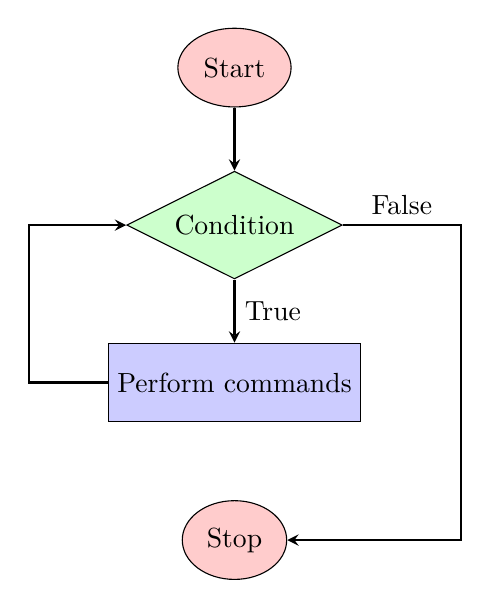
\begin{tikzpicture}
                \node (start) [startstop] {Start};
                \node (cond) [decision, below of=start, yshift=-1cm] {Condition};
                \node (command) [process, below of=cond, yshift=-1cm] {Perform commands};
                \node (stop) [startstop, below of=command, yshift=-1cm] {Stop};

                \draw [arrow] (start) -- (cond);
                \draw [arrow] (cond) -- (command) node[midway, right] {True};
                \draw [arrow] (command.west) -- ++(-1, 0) |- (cond);
                \draw [arrow] (cond.east) -- node[midway, above] {False} ++(1.5, 0) |- (stop);
            \end{tikzpicture}
        \end{column}
        \begin{column}{0.5\textwidth}
            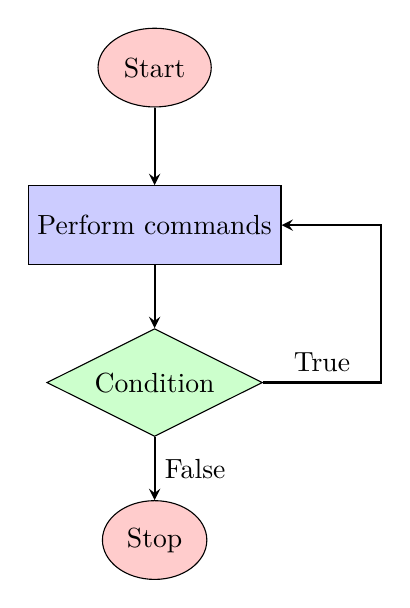
\begin{tikzpicture}
                \node (start) [startstop] {Start};
                \node (command) [process, below of=start, yshift=-1cm] {Perform commands};
                \node (cond) [decision, below of=command, yshift=-1cm] {Condition};
                \node (stop) [startstop, below of=cond, yshift=-1cm] {Stop};

                \draw [arrow] (start) -- (command);
                \draw [arrow] (command) -- (cond);
                \draw [arrow] (cond.east) -- ++(1.5, 0) node[midway, above] {True} |- (command.east);
                \draw [arrow] (cond) -- (stop) node[midway, right] {False};
            \end{tikzpicture}
        \end{column}
        \end{columns}
    \end{frame}


    \section{\texttt{break} and \texttt{continue}}

    \begin{frame}{The \texttt{break} Statement}
        \begin{itemize}
            \item The break statement immediately terminates the loop or switch statement in which it is encountered
            \item Control of the program then transfers to the statement immediately following the loop or switch
            \item It is commonly used to exit a loop prematurely based on a certain condition
        \end{itemize}
    \end{frame}


    \begin{frame}[fragile]{\texttt{break} Example}
        \inputminted[
            frame=none,
            bgcolor=gray!20,
            linenos, 
            breaklines=true,
            fontsize=\fontsize{12pt}{13pt}\selectfont
        ]{c}{../code-examples/06_13_break.c}
    \end{frame}


    \begin{frame}{The \texttt{continue} Statement}
        \begin{itemize}
            \item The continue statement skips the remaining statements in the current iteration of a loop and proceeds to the next iteration
            \item It is used when you want to bypass certain parts of the loop's body for specific conditions without exiting the entire loop
        \end{itemize}
    \end{frame}


    \begin{frame}[fragile]{\texttt{continue} Example}
        \inputminted[
            frame=none,
            bgcolor=gray!20,
            linenos, 
            breaklines=true,
            fontsize=\fontsize{12pt}{13pt}\selectfont
        ]{c}{../code-examples/06_14_continue.c}
    \end{frame}


    \section{Nested Loops}


    \section{The \texttt{switch} Statement}


    \section{Exercise}

    \begin{frame}[allowframebreaks=0.75]{Exercise}
        Write C programs:
        \begin{enumerate}
            \item To check whether a number (user input) is positive or negative or zero
            \item To check whether a year (user input) is a leap year
            \item To check whether an integer is even or odd
            \item To find the number of real-valued solution(s) to a quadratic equation, (\(ax^2+bx+c=0\)). Take \texttt{a}, \texttt{b} and \texttt{c} as user inputs. Then calculate the value of the discriminant, then show the appropriate output
            \item To print the first n (user input) natural numbers using a \texttt{for} loop. And another program to do the same using a \texttt{while} loop
            \item To compute the sum of numbers from 1 to n using a \texttt{for} loop. And another program to do the same using a \texttt{while} loop
            \item To find the factorial of an intger (user input)
            \item To print the first n (user input) terms of the fibonacci series
            \item To print the first n (user input) terms of the following arithmetic progression sequence: 1, 4, 7, 10, 13\dots
            \item To repeatedly take user input and print its square, until a negative number is entered (use while loop)
            \item To repeatedly take user input as exam marks and print the corresponding letter grade, until a negative number is entered (use \texttt{while} loop and \texttt{if} statement)
            \item To find the GCD of two integers using the Euclidean algorithm
            \item To find the LCM of two integers
        \end{enumerate}
    \end{frame}

\end{document}
